\section{Sumas ortogonales de espacios de Hilbert}

\TODO{Me parece que nunca hago referencia a esta sección
para la tesis! La necesitaba para lo que ahora será
parte de la de maestría. La quito entonces?}


\begin{defi} \label{def: suma ortogonal finita de subespacios ortogonales dos a dos}
Sean $V$ un espacio de Hilbert, 
$\{ V_{j} \}_{j=1}^{n}$ una familia de subespacios cerrados
de $V$. Si ocurre que para índices distintos 
$i,j \in \Delta$ los espacios correspondientes
$V_{i}$ y $V_{j}$ son ortogonales entre sí (o, equivalentemente,
que uno esté contenido en el complemento ortogonal
del otro), entonces
diremos que la familia es 
\textbf{ortogonal dos a dos}. Además, a la suma
de estos espacios (que es un subespacio de $V$)
la denotaremos por
\[
\ameboxplus_{j =1 }^{n} V_{j},
\]
y la llamaremos \textbf{suma ortogonal de la familia}
$\{ V_{j} \}_{j=1}^{n}$.
\end{defi}

Es fácil observar que la suma de una familia finita
ortogonal dos a dos $\{ V_{j} \}_{j=1}^{n}$
es de hecho una suma directa
de subespacios (en el sentido dado por [\TODO{referencia. Rotman}]);
si $v_{1} + \cdots +v_{n}$, con $v_{j} \in V_{j}$
para toda $j$, es el vector cero de $V$, entonces

\begin{align*}
0 =  & < v_{j} , \suma{i=1}{n}{v_{i}} > \\
& = \suma{i=1}{n}{<v_{j} , v_{i}>} \\
& =< v_{j} , v_{j} > = || v_{j} ||^{2},
\end{align*}
o sea, todos los sumandos $v_{j}$
son el vector cero. \\

\begin{prop} \label{prop: pasar de resta ortogonal a suma ortogonal}
Sean $V$ un espacio de Hilbert, $W$ y $Z$ dos subespacios
de $V$, con $Z$ cerrado en $V$ y $Z \subseteq W$.
Si $U$ se define como el espacio $W \cap Z^{\perp}$, 
o sea, si 
\[
U:= W \boxminus Z,
\]
entonces 
\[
W= U \boxplus Z.
\]
\end{prop}
\noindent
\textbf{Demostración.}
Como $U$ está contenido en $Z^{\perp}$, 
claro que la suma de los espacios es ortogonal.
Además, el que esta esté contenida en $W$ es obvio,
pues tanto $U$ como $Z$ están contenidos en $W$
(lo primero por construcción de $U$ y lo 
segundo por hipótesis) y $W$ es 
cerrado bajo sumas.

Sea ahora $a \in W$ cualquiera. 
Como $Z$ es cerrado, podemos proyectar sobre él (c.f. teorema
\ref{Teo:proyOrt}); consideremos entonces al vector
$\Pi_{Z}(w)$; tenemos que
\[
w= (w-\Pi_{Z}(w))+\Pi_{Z}(w),
\]
donde
\begin{itemize}
\item $ w \in W$ y $\Pi_{Z}(w) \in Z \subseteq W$, por lo tanto
$w-\Pi_{Z}(w) \in W$, y
\item $\Pi_{Z}(w) \in Z$.
\end{itemize}
\QEDB
\vspace{0.2cm}

\begin{lema} \label{lema: BONs de sumas ortogonales}
(personal): Sea $\{ V_{j} \}_{j=1}^{n}$ una familia
de subespacios cerrados del espacio de Hilbert $V$ ortogonales
dos a dos. 
\begin{itemize}
\item Si $\cali{B}$ es una BON de $\ameboxplus_{j =1 }^{n} V_{j}$,
entonces, para todo índice $j$,
\[
\cali{B}_{j}:= \cali{B} \cap V_{j}
\]
es una BON de $V_{j}$. 

\item Si para cada $j$, $\cali{B}_{j}$ es una
BON de $V_{j}$, entonces

\[
\cali{B}:= \union{j=1}{n}{\cali{B}_{j}}
\]
es una BON de $\ameboxplus_{j =1 }^{n} V_{j}$.
(compare esto con el que, en una suma directa
de espacios vectoriales, la union de bases es base de Hamel de esta
\TODO{AA. establece bien la analogía})
\end{itemize}
\end{lema}
\noindent
\textbf{Demostración.} La prueba consiste en usar
repetidas veces la equivalencia AA 
establecida en \TODO{THM 4.13 Conway}.
\begin{itemize}
\item Sea $j$ un índice. 
Sea $v_{j} \in V_{j}$ tal que 
\begin{equation} \label{eq 1:lema BON de sumas ortogonales}
(\forall w \in \cali{B}_{j}):
\hspace{0.5cm} <w, v_{j}>=0;
\end{equation}


mostremos que entonces $v_{j} =0$. Según el 
\TODO{THM 4.13 Conway}, esto bastará para demostrar que
$\cali{B}_{j}$, que es un subconjunto ortonormal
del espacio $V_{j}$, es BON de este. \\
Observe que, como la familia $\{ V_{j} \}_{j=1}^{n}$
es ortogonal dos a dos y $v_{j} \in V_{j}$,
\begin{equation} \label{eq 2:lema BON de sumas ortogonales}
(\forall w \in \cali{B}- \underbrace{\cali{B}_{j}}_{\text{la
parte de } \cali{B} \text{ en } V_{j}}): \hspace{0.5cm}
<w, v_{j}>=0.
\end{equation}

Las proposiciones \eqref{eq 1:lema BON de sumas ortogonales}
y \eqref{eq 2:lema BON de sumas ortogonales}
juntas significan que
\[
\forall w \in \cali{B}: <w, v_{j}>=0;
\]
como $\cali{B}$ es BON de $\ameboxplus_{j =1 }^{n} V_{j}$,
esto último implica, según \TODO{THM 4.13 Conway},
que $v_{j}$ es cero.



\item Si mostramos
que el único $v=v_{1} + \cdots + v_{n} \in \ameboxplus_{j =1 }^{n} V_{j}$
ortogonal a todo elemento de $\cali{B}$ 
es el vector cero, podremos concluir según \TODO{THM 4.13 Conway}
que $\cali{B}$ es una BON de la suma directa.
Sea $j$ un índice cualquiera. Puesto que
$\cali{B}_{j} \subseteq \cali{B}$, tenemos que
\[
(\forall b \in \cali{B}_{j}): 
0=<v,b> = <v_{1} + \cdots + v_{n}, b> = <v_{j}, b>,
\]
dándose la última igualdad por ser $b$ un elemento de 
de $V_{j}$ y las $v_{i}$ con $i \neq j$ elementos
de los espacios $V_{i} \subseteq V_{j}^{\perp}$.
Según esto último, $v_{j}$ es un elemento de $V_{j}$
ortogonal a todo elemento de la BON $\cali{B}_{j}$ 
de $V_{j}$; así, 
según el \TODO{THM 4.13 Conway} $v_{j}=0$. 
Concluimos que
\[
v=0 + \cdots + 0=0.
\]

\end{itemize}
\QEDB
\vspace{0.2cm}



\begin{lema} \label{lema: proyección sobre la suma ortogonal}
 (personal)
Sea $\{ V_{j} \}_{j=1}^{n}$ una familia
de subespacios cerrados del espacio de Hilbert $V$ ortogonales
dos a dos.
Para todo $v \in V$, 
\[
\Pi_{\ameboxplus_{j =1 }^{n} V_{j}}(v)
= \suma{j=1}{n}{\Pi_{V_{j}}(v)}
\]
\end{lema}
\noindent
\textbf{Demostración.}
Para cada índice $j$ sea $\cali{B}_{j}$ una
BON de $V_{j}$. 

Por el lema \ref{lema: BONs de sumas ortogonales}, sabemos
que $\cali{B}:= \union{j=1}{n}{\cali{B}_{j}}$
es una BON de la suma ortogonal.

Según \TODO{EX conway},
para toda $j$,
\[
\Pi_{V_{j}}(v)= \suma{}{}{\{ <v, e_{j}> | e_{j} \in \cali{B_{j}} \}}.
\]

Sea $\epsilon>0$ cualquiera. Por definición de convergencia
de redes, existen $G_{j} \subseteq \cali{B}_{j}$
finitos tales que
\begin{equation} \label{eq 1: lema: proyección sobre la suma ortogonal}
G_{j} \underbrace{\subseteq}_{\text{finito}} F_{j} \hspace{0.2cm}
\Rightarrow \hspace{0.4cm}
|| \Pi_{V_{j}}(v)- \suma{i \in F_{j}}{}{<v, e_{i}>e_{i}}  || < 
\frac{\epsilon}{n};
\end{equation}


así, $G:=\union{j=1}{n}{G_{j}}$ es un subconjunto finito de 
$\cali{B}$ (pues es unión finita de finitos) tal que,
si $G\underbrace{\subseteq}_{\text{finito}} F$
y $F_{j} := F \cap \cali{B}_{j}$, entonces, 
como
\[
F_{j} = F \cap \cali{B}_{j} \supseteq 
G \cap \cali{B}_{j} = G_{j}
\]

según la implicación 
\eqref{eq 1: lema: proyección sobre la suma ortogonal}
 y la desigualdad triangular, 
\begin{align*}
|| \suma{j=1}{n}{\Pi_{V_{j}}(v)} - \suma{i \in F}{}{<v, e_{i}>e_{i}} ||
\leq &  \suma{j=1}{n}{||\Pi_{V_{j}}(v)- \suma{i \in F_{j}}{}{<v, e_{i}>e_{i}}||} \\
\leq & n \cdot \frac{\epsilon}{n} = \epsilon.
\end{align*}

De la unicidad del límite de una red
y una segunda aplicación del \TODO{EX Conway}
se concluye que

\[
\suma{j=1}{n}{\Pi_{V_{j}}(v)} = 
\suma{}{}{\{ <v, e> | e \in \cali{B} \}} = \Pi_{\ameboxplus_{j =1 }^{n} V_{j}}(v).
\]

\begin{figure}[H]
	\sidecaption{
	Por ejemplo, sea $V= \IR^{3}$ con el producto
	punto usual, y sean  $X$, $Y$ y $Z$ los ejes
	$x$, $y$ y $z$, respectivamente.
	Estos son subespacios cerrados de $V$ mutuamente ortogonales. Como
	se muestra gráficamente, la proyección de $v$ al plano $XY$
	(que es la suma de $X$ con $Y$) coincide con la suma
	de las proyecciones a $X$ y a $Y$.
	\label{fig: proyecciones sumas}}
	\centering
	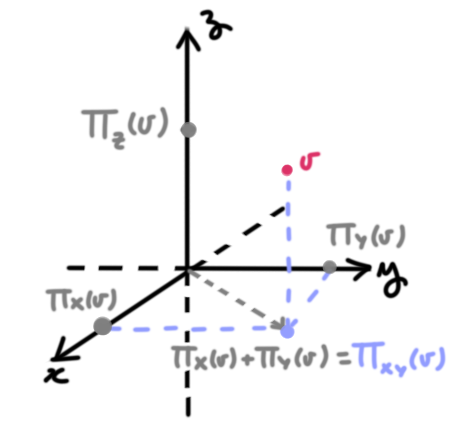
\includegraphics[scale=1.7]{31Julio_1} 
\end{figure}	



\QEDB
\vspace{0.2cm}


\begin{prop} \label{prop: elemento de la suma ortogonal de subespacios}
Si $\{ V_{j} \}_{j=1}^{n}$ es una familia de subespacios 
cerrados
ortogonales dos a dos
y $v \in \ameboxplus_{j =1 }^{n} V_{j}$, entonces los (únicos) elementos
de los espacios $V_{j}$ que sumados son iguales a $v$
son las proyecciones de $v$ sobre estos:

\[
v = \suma{j=1}{n}{ \Pi_{V_{j}}(v)}.
\]
\end{prop}
\noindent
\textbf{Demostración.}
Sea $\cali{B}$ una BON para la suma directa; por el lema 
\ref{lema: BONs de sumas ortogonales}, sabemos que,
para cada $j$,
\[
\cali{B}_{j}:= \cali{B} \cap V_{j}
\]
es una BON para $V_{j}$.

Por ser la suma de estos espacios directa, sabemos
que existen únicos $v_{j} \in V_{j}$ tales que
\[
v=v_{1} + \cdots + v_{n}.
\]
Por el \TODO{THM 4.13, Conway},

\begin{equation}
\label{eq 1:prop elemento de la suma ortogonal de subespacios}
v_{j}= \suma{}{}{\{ <v_{j},e> | e \in \cali{B}_{j}  \}}.
\end{equation}


Observe ahora que
\begin{equation}
\label{eq 2:prop elemento de la suma ortogonal de subespacios}
\suma{}{}{\{ <v_{j},e> | e \in \cali{B}_{j}  \}}=
\suma{}{}{\{ <v,e> | e \in \cali{B}_{j}  \}};
\end{equation}

en efecto, 
esto se deduce de inmediato del notar que,
para toda $e \in \cali{B}_{j}$,
\begin{align*}
<v, e> = & <v_{1} + \cdots + v_{n}, e> \\
= & <v_{1}, e> + \cdots + <v_{n}, e> \\
= & <v_{j}, e> 
\end{align*}
(dándose la última igualdad por ser $e \in V_{j} \subseteq V_{i}^{\perp}$
ortogonal a todos los $v_{i} \in V_{i}$ con $i \neq j$.) \\

Ahora bien, según el corolario \TODO{Ex. 13 conway},
\begin{equation}
\label{eq 3:prop elemento de la suma ortogonal de subespacios}
\suma{}{}{\{ <v,e> | e \in \cali{B}_{j}  \}}= \Pi_{V_{j}}(v).
\end{equation}

Juntando lo establecido en las igualdades
\eqref{eq 1:prop elemento de la suma ortogonal de subespacios},
\eqref{eq 2:prop elemento de la suma ortogonal de subespacios} y
\eqref{eq 3:prop elemento de la suma ortogonal de subespacios}
llegamos, como queríamos, a que
$v_{j}= \Pi_{V_{j}}(v).$

\QEDB
\vspace{0.2cm}


\begin{defi}
Si $\{ V_{j} \}_{j \in \IN}$ es una familia 
numerable de subespacios cerrados
de $V$ ortogonales dos a dos, definimos
a $\ameboxplus_{j \in \Delta} V_{j}$ como el siguiente
subespacio cerrado de $V$:
\begin{align*}
\ameboxplus_{j \in \IN} V_{j} := & \hspace{0.2cm}
\overline{\{ v_{1}+ \ldots + v_{n} :
n \in \IN, v_{j} \in V_{j}
\hspace{0.4cm} \text{para toda} \hspace{0.2cm} j \}} \\
= & \hspace{0.2cm} \overline{\union{n \in \IN}{}{\suma{j=1}{n}{V_{j}}}}
= \hspace{0.2cm} \overline{\union{n \in \IN}{}{\ameboxplus_{j=1}^{n} V_{j}}} .
\end{align*}
\end{defi}


\begin{prop} \label{prop: caracterizacion suma infinita de subespacios ortogonales} 
Con los elementos de la definición anterior,
$ v \in \ameboxplus_{j \in \IN} V_{j} $
si y sólo si existe $(v_{j})_{j \in \IN}$ 
elemento del producto cartesiano de la familia 
$\{ V_{j} \}_{j \in \IN}$
\footnote{i.e. una sucesión
de $V$, con $v_{j} \in V_{j}$ para toda $j$}
tal que 
\begin{itemize}
\item $v = \suma{j=1}{\infty}{v_{j}}$ y
\item $\suma{j=1}{\infty}{|| v_{j} ||^{2}}< \infty $.
\end{itemize}
De hecho, $(v_{j})_{j \in \IN}$ es el único elemento
del producto cartesiano de la familia cuya sucesión de
sumas parciales converge a $v$. Además, se tiene la igualdad
$|| v ||^{2}= \suma{j=1}{\infty}{|| v_{j} ||^{2}} $.
\end{prop}
\noindent
\textbf{Demostración.}
\begin{itemize} 
\item[$\Leftarrow$)] Es claro cómo el que exista una tal
sucesión $(v_{j})_{j \in \IN}$ ya implica que $v$ sea
elemento de $ \ameboxplus_{j \in \IN} V_{j} $ pues,
dado $\epsilon >0$ cualquiera, por definición de convergencia 
de series existe un $n \in \IN$ tal que
\[
| v - \suma{j=1}{n}{v_{j}} | < \epsilon . 
\]
\item[$\Rightarrow$)]  Sea $v \in \ameboxplus_{j \in \IN} V_{j} $;\\
(Existencia)
Si mostramos que
\[
v = \limite{J \rightarrow \infty}{v_{J}}, \hspace{0.4cm}
\text{donde} \hspace{0.2cm} v_{J}:= \Pi_{\ameboxplus_{j =1}^{J} V_{j}}(v),
\]
puesto que según el lema \ref{lema: proyección sobre la suma ortogonal}
$v_{J}= \suma{j=1}{J}{\Pi_{V_{j}}(v)}$,
tendremos que el elemento \[
\left( \Pi_{V_{j}(v)} \right)_{j \in \IN}
\]
del producto cartesiano de la familia
es tal que
\[
\suma{j=1}{\infty}{\Pi_{V_{j}}(v)}
= \lim_{J \rightarrow \infty} \suma{j=1}{J}{\Pi_{V_{j}}(v)}
= \limite{J \rightarrow \infty}{v_{J}}=v.
\]


Supongamos pues que existe $\epsilon >0$
para el que no sea posible hallar un $J>0$ tal que
$| v - v_{J} | < \epsilon $. Por definición del espacio 
$\ameboxplus_{j \in \IN} V_{j}$, sí que existen $J>0$
y $v_{j} \in V_{j}$, con $1 \leq j \leq J$ 
tales que $|v - \suma{i=1}{J}{v_{i}}| < \epsilon $; hemos
hallado así al elemento $\suma{i=1}{J}{v_{i}}$ de 
$\ameboxplus_{j =1}^{J} V_{j}$
tal que
\[
|v - \suma{i=1}{J}{v_{i}} | < \epsilon \leq |v - v_{J}| 
= |v - \Pi_{\ameboxplus_{j =1}^{J} V_{j}}(v) |,
\]

contradiciendo la definición del vector 
$\Pi_{\ameboxplus_{j =1}^{J} V_{j}}(v)$.



(Unicidad) Sea ahora
$(a_{j})$ elemento del producto cartesiano tal que $\suma{j=1}{\infty}{a_{j}}=0$.
Tenemos la siguiente cadena de igualdades;
\begin{align*}
0 = <0,0> = & < \suma{j=1}{\infty}{a_{j}} , \suma{j=1}{\infty}{a_{j}}  > \\
= & < \limite{n \rightarrow \infty}{\suma{j=1}{n}{a_{j}}},
\limite{n \rightarrow \infty}{\suma{j=1}{n}{a_{j}}}> \\
\text{(por proposición \ref{prop: continuidad del producto punto})}
= & \limite{n \rightarrow \infty}{ \langle \suma{j=1}{n}{a_{j}}  ,
\suma{j=1}{n}{a_{j}} \rangle }  \\
\text{(por ortogonalidad)}= & \limite{n \rightarrow \infty}{\suma{i=1}{n}{|| a_{i}||^{2}}};
\end{align*}
deducimos a partir de ella que la norma de cada $a_{j}$ es cero;
así, el suponer $\suma{j=1}{\infty}{a_{j}}=0$ implica la igualdad
a cero de cada
$a_{j}=0$.  De esto deducimos que, para todo 
$v \in \ameboxplus_{j \in \IN} V_{j}$, si $(v_{j})$ y $(w_{j})$
son dos
elementos del producto cartesiano para los que
$\suma{j=1}{\infty}{v_{j}}=v = \suma{j=1}{\infty}{w_{j}}$,
entonces
\[
\suma{i=1}{\infty}{(v_{j}-w_{j})}= 
\suma{j=1}{\infty}{v_{j}} - \suma{j=1}{\infty}{w_{j}} = v-v=0,
\]
de donde $v_{j}=w_{j}$. \\

Mostremos por último que $|| v ||^{2} = \suma{i=1}{\infty}{|| v_{i} ||^{2}} $.
Por la bilinealidad del producto punto y
y la ortogonalidad de los subespacios, para toda $n \in \IN$
\[
< v_{1}+ \ldots + v_{n} , v_{1}+ \ldots + v_{n}  > =
< v_{1} , v_{1} > + \ldots + < v_{n} , v_{n} >,
\]
luego,
\begin{align*}
\suma{i=1}{\infty}{||v_{i}||^{2}} = &
\limite{n \rightarrow \infty}{\suma{i=1}{n}{||v_{i}||^{2}}} \\
= & \limite{n \rightarrow \infty}{\langle 
\suma{i=1}{n}{v_{i}} , \suma{i=1}{n}{v_{i}} \rangle };
\end{align*}
por la continuidad establecida en la 
proposición \ref{prop: continuidad del producto punto},
podemos continuar la cadena de igualdades como sigue:
\begin{align*}
\suma{i=1}{\infty}{||v_{i}||^{2}} = & \langle  \limite{n \rightarrow \infty}{\suma{i=1}{n}{v_{i}}} ,
 \limite{n \rightarrow \infty}{\suma{i=1}{n}{v_{i}}} \rangle \\
 & = < v , v > = ||v||^{2}.
\end{align*}
\end{itemize}
\QEDB
\vspace{0.2cm}
\newpage